\documentclass{beamer}

\usepackage{fontspec} 
% \usepackage{lsp-makros}
\useoutertheme{lsp}

\usepackage{lsptitle}

\def\two@digits#1{\ifnum#1<10 0\fi\number#1}
\def\mytoday{\two@digits{\number\day}.\two@digits{\number\month}.\number\year}


\usepackage{xspace,multicol}
\newcommand{\latex}{\LaTeX\xspace}
\usepackage{tikz}


\newcounter{lastpagemainpart}
\footnotesep0pt
\renewcommand{\footnoterule}{}
\usefootnotetemplate{
  \noindent
  \insertfootnotemark\insertfootnotetext}

\let\beamerfn=\footnote
\renewcommand{\footnote}[1]{%
\let\oldfnsize=\footnotesize%
\let\footnotesize=\tiny%
\beamerfn<\thebeamerpauses->{#1}%
\let\footnotesize=\oldfnsize}


\date{\today}

\usepackage{eurosym}  
 
\renewcommand{\centerline}[1]{\hfill#1\hfill\hfill\mbox{}}


\title{Series Editors' Meeting 2017}
% \institute{FU Berlin}
\author[LangSci]{Sebastian Nordhoff}



\begin{document}
\lspbeamertitle


\section{Books} 
\frame{
\frametitle{Published works} 
      
\includegraphics[width=1.2cm]{bisang.png}
~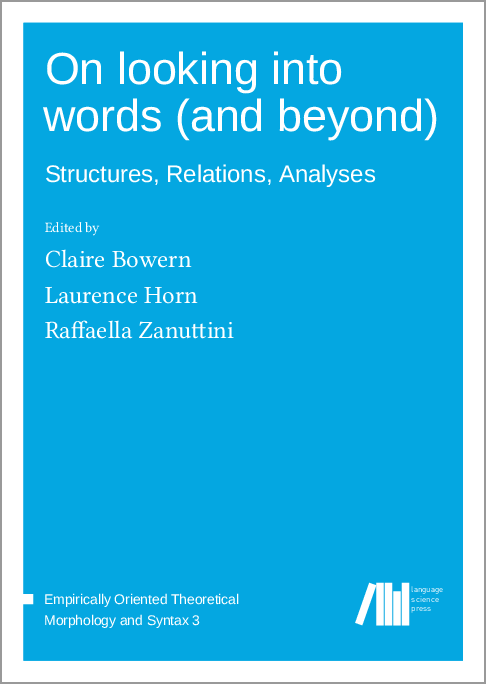
\includegraphics[width=1.2cm]{bowern.png}
~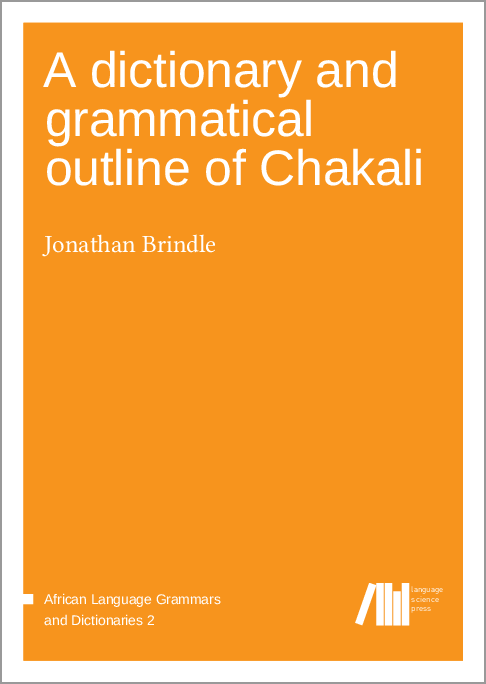
\includegraphics[width=1.2cm]{brindle.png}
~
\includegraphics[width=1.2cm]{enfield.png}
 %                            124
~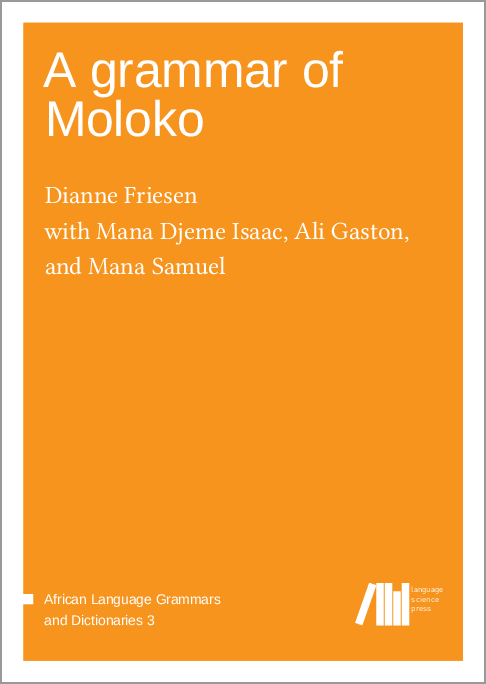
\includegraphics[width=1.2cm]{friesen.png}
~
\includegraphics[width=1.2cm]{kieviet.png}
~
\includegraphics[width=1.2cm]{klamer.png}
~
\includegraphics[width=1.2cm]{kluge.png}

  %                           124

\includegraphics[width=1.2cm]{menzel.png}
~
\includegraphics[width=1.2cm]{michaud.png}
~
\includegraphics[width=1.2cm]{payne.png}
~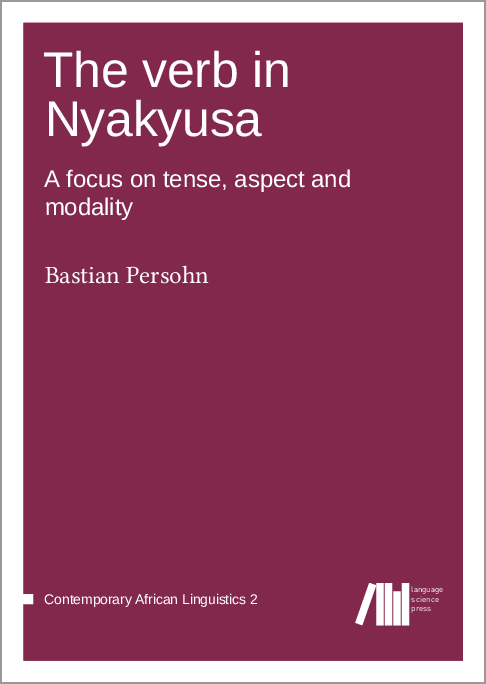
\includegraphics[width=1.2cm]{persohn.png}
 %                            124
~
\includegraphics[width=1.2cm]{roettger.png}
~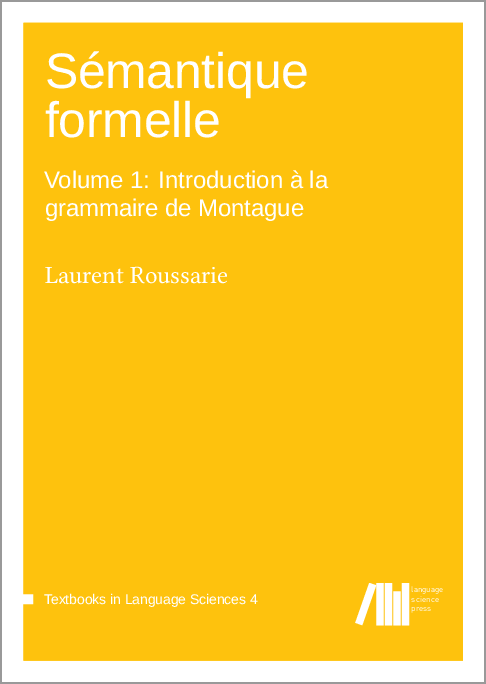
\includegraphics[width=1.2cm]{roussarie.png}
~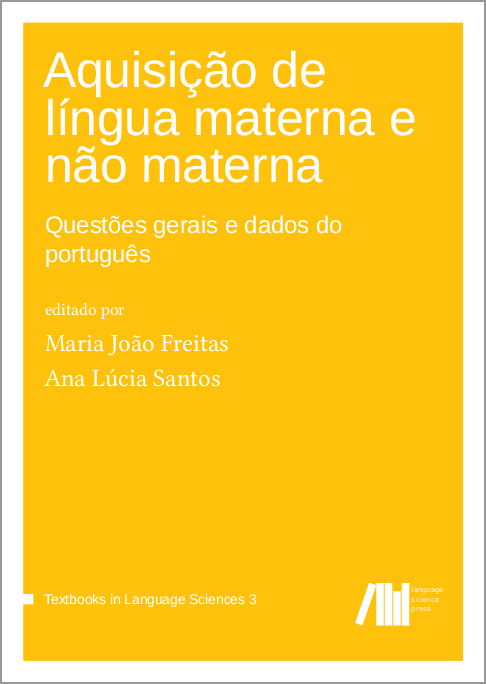
\includegraphics[width=1.2cm]{santos.png}
~
\includegraphics[width=1.2cm]{schaefer.png}

   %                          124

\includegraphics[width=1.2cm]{schrock.png}
~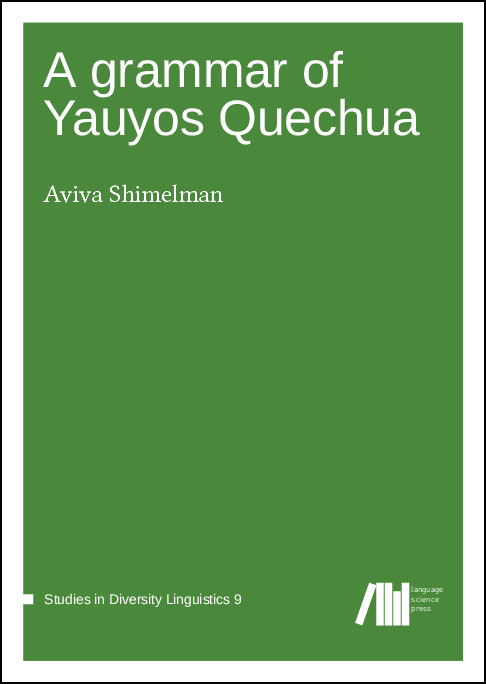
\includegraphics[width=1.2cm]{shimelman.png}
~
\includegraphics[width=1.2cm]{song.png}
~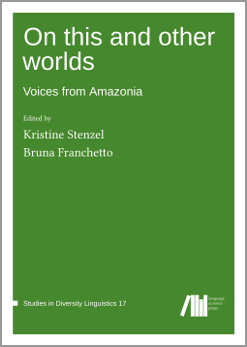
\includegraphics[width=1.2cm]{stenzel.png}                              
~
\includegraphics[width=1.2cm]{tc3ii.png}
~
\includegraphics[width=1.2cm]{tc3i.png}
~
\includegraphics[width=1.2cm]{trips.png}
~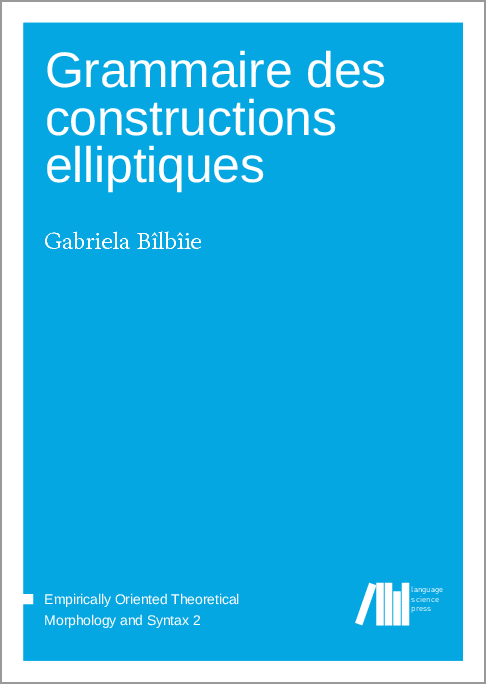
\includegraphics[width=1.2cm]{bilbiie.png}
\begin{itemize}
 \item projected for 2018: 30 works, but already 36 in the pipeline
\end{itemize}

}

\frame{
\frametitle{}
\begin{itemize}
 \item Expressions of interest in 2017: 80 (2016: 73)
 \item duration of publication
 \begin{itemize}
  \item reviewing: 91 days median, 253 days max
  \item submission$\to$publication: 244d median, 1145d max
 \end{itemize}
\end{itemize}
}

\frame{
\frametitle{Downloads since 2014}
\begin{itemize}
 \item total edited volumes: 61,825
 \item total monographs: 89,340
 \item Tonal placement in Tashlhiyt 178 $\leftrightarrow$ The future of dialects 20,913
\end{itemize}

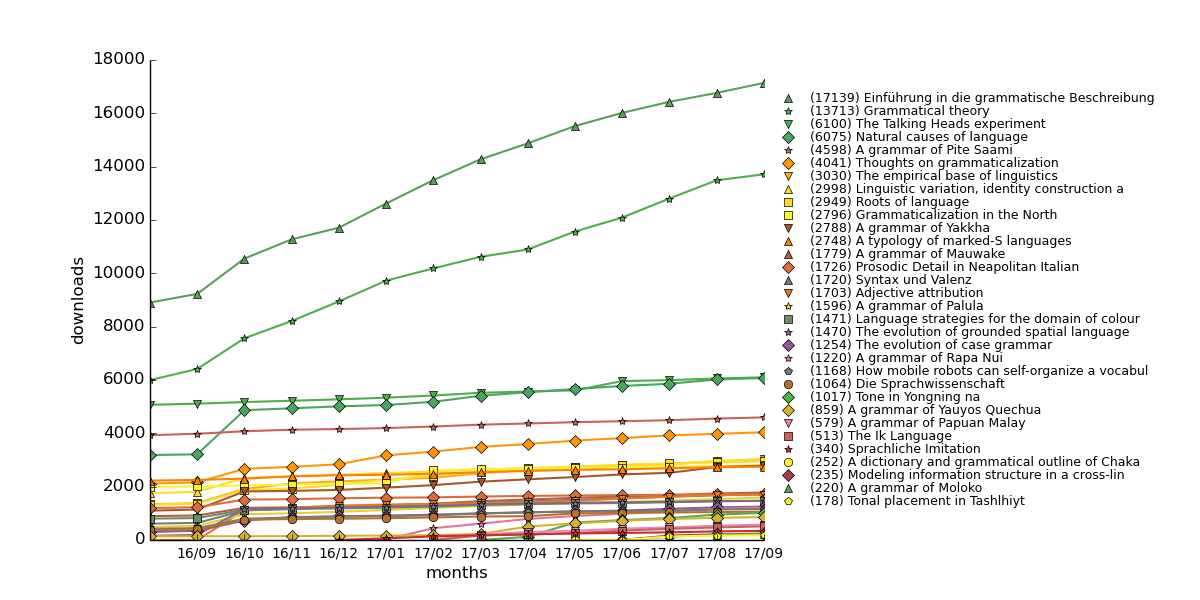
\includegraphics[height=.8\textheight]{cumulativeallmonograph.png}

}




\frame{
\frametitle{Print}
\begin{itemize}
 \item change of service provider from CreateSpace to BoD
 \item worldwide, softcover, cheap, easier handling, no customs issues 
\end{itemize}
}

\section{Community} 
\frame{
\frametitle{Community}
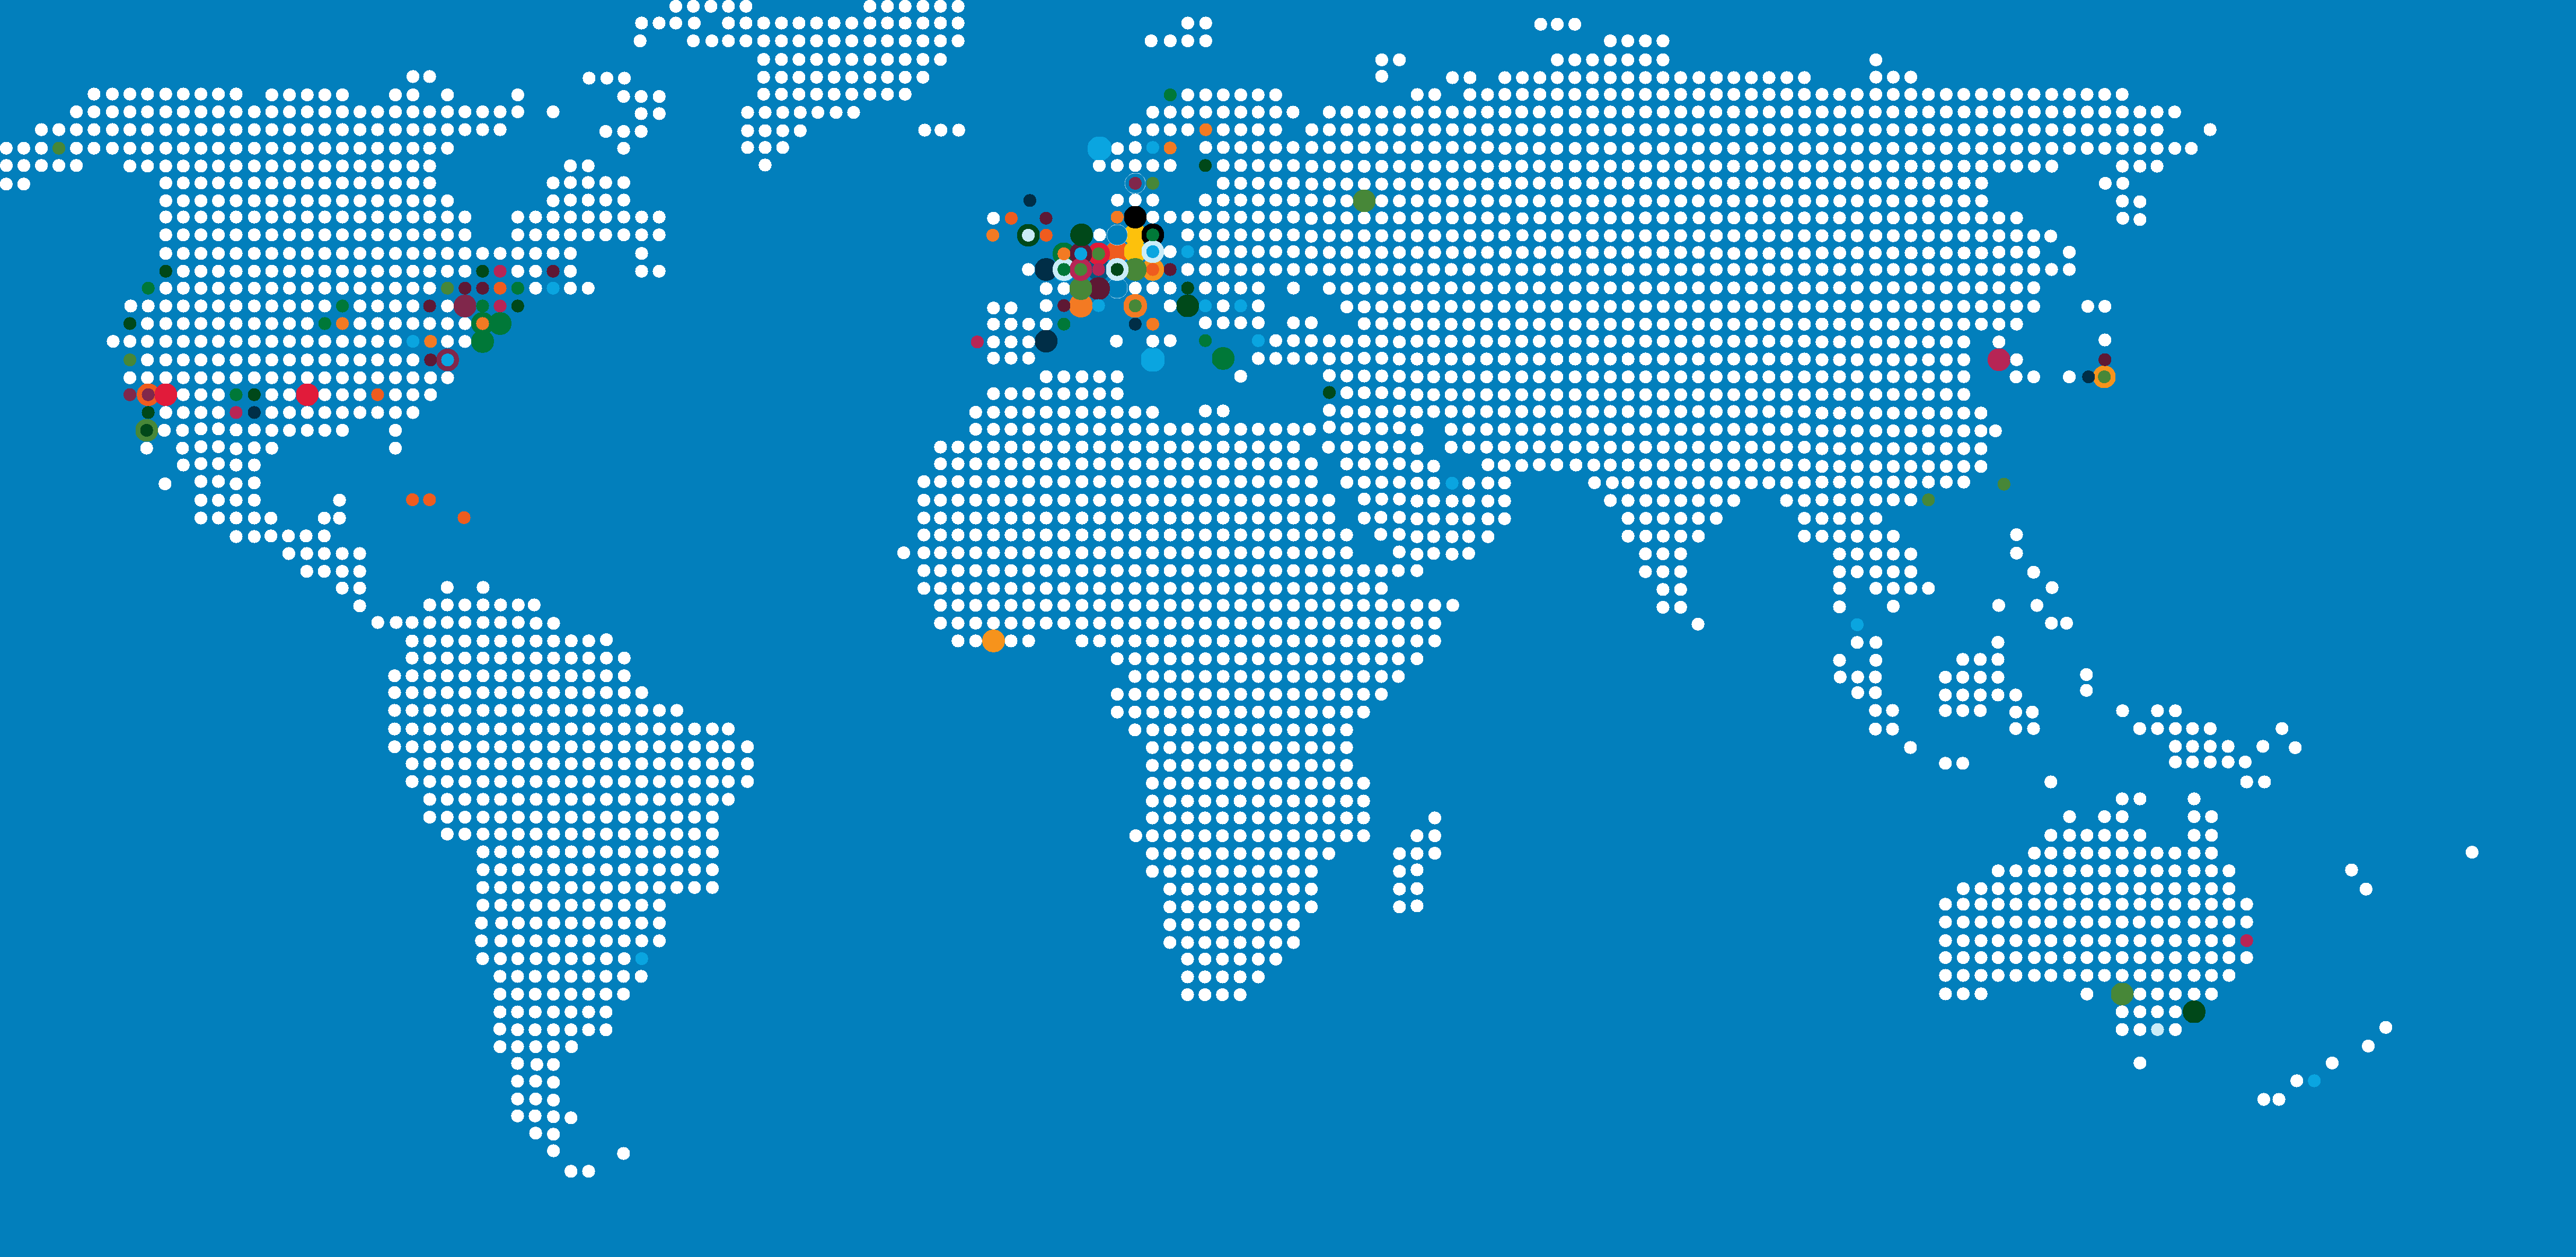
\includegraphics[height=.8\textheight]{WORLDMAPDOTSdots.png}
\begin{itemize}
 \item well distributed
 \item not all equally responsive
 \item 1269 OMP users, 916 supporters
 \item 1297 Twitter followers, 1324 Facebook followers
\end{itemize}
}

\frame{
\frametitle{Staff}
\begin{itemize}
 \item 1 coordinator
 \item 1 student assistant \pause 
 \item about 300 volunteers 
\end{itemize}
}
    
    
\section{IT}
\frame{
\frametitle{IT}
\begin{itemize}
 \item Zenodo used as a DOI provider 
 \item Paperhive now used for all proofreading 
 \begin{itemize}
  \item  now regularly over 1000 comments in proofreading
  \item   unbalance between typology++ and the rest
\end{itemize}
 \item all books directly linked from LangSci site
 \item \raisebox{-.37em}{
\includegraphics[height=1.5em]{docloop.png}} for backlink from Paperhive to author
\end{itemize}

}
 
\section{Outreach}
\frame{
\frametitle{Conferences/workshops}
\begin{itemize}
 \item Open-Access-Tage, Dresden
 \item FID Afrikanistik, Frankfurt/M
 \item Middle Eastern Studies, Marburg 
 \item Verband der Philologie-Fachreferaten NRW, Bergisch-Gladbach 
 \item Ministry for Research and Education, Berlin 
 \item Deutsche Forschungsgemeinschaft, Bonn  Allianz-Initiative Digitale Information, AG  Wissenschaftliches Publikationswesen
\end{itemize}
} 

\section{Funding}

\frame{
\frametitle{Funding as of today}
\begin{itemize}
 \item Knowledge Unlatched
 \begin{itemize}
  \item 69/100 institutions @ 1,000 EUR
  \item 3/150 individual pledges  @ 100 EUR
 \end{itemize}
 \item Book processing charges
 \begin{itemize}
  \item 1 * 1,500 EUR; 1 * 1,000 EUR
 \end{itemize}
  \item print margin total: 3,500 EUR
  \item {\color{red} short ca. 40,000 EUR p/a as compared to projected costs of 115,000 EUR}
  \item not sustainable in the long run
\end{itemize}
}    

\section{Today}

\frame{
\frametitle{Agenda for today}
\begin{itemize}
 \item experiences in the past year
\begin{itemize}
 \item monographs
 \item  edited volumes  
\end{itemize}
\item best practices
\begin{itemize}
 \item acquiring manuscripts
 \item finding reviewers
 \item timelines
 \item conversion process
 \item bibliographies
 \item proofreading process
 \item dealing with demanding authors/volume editors
\end{itemize}
 \rule{10cm}{1pt}
 \item Lunch\\[-.4em]
 \rule{10cm}{1pt}
  
 
 \item Future funding 
 \item Future setup
\end{itemize}
}

\end{document}